\paragraph{5.1} \textbf{Transformation is Unitary}
\\

$$U|j\rangle = \frac{1}{\sqrt{N}} \sum_{k=0}^{N-1} e^{{2 \pi \iota j k}/N} |k\rangle$$

$$ \langle j^{\prime} |U^{\dagger} U | j \rangle = \frac{1}{N} \sum_{k=0}^{N-1} e^{2\pi \iota (j-j^{\prime}) k/N}$$

Case 1: $\Delta j = j - j^{\prime} = 0 \implies P = 1$

\\

Case 2: $\Delta j = j - j^{\prime} \ne 0$

$$ \frac{1}{N} \sum_{k=0}^{N-1} r^{k} \ \ (r = e^{2 \pi \iota \Delta j/N})$$

$$ \frac{1-r^N}{1-r} = \frac{1-e^{2\pi \iota \Delta j}}{1-r} = 0$$
$( \Delta j \in \mathbb{Z})$

$$ U^{\dagger} U = 1$$

\paragraph{5.2} \textbf{Compute the Fourier Transform}

$$U|00...0\rangle = \frac{1}{\sqrt{2^{n}}} \sum_{i_1,...i_n} |i_1....i_n\rangle$$

\paragraph{5.4} \textbf{Give a Decomposition}
\\

The controlled $R_k$ gate, where $k$ is an integer, can be decomposed into a sequence of single qubit gates and CNOT gates. One way to decompose it is as follows:
\begin{itemize}
    

\item  Apply a Hadamard gate (H) to the control qubit.
\item Apply a Rk gate to the target qubit.
\item Apply a CNOT gate with the control qubit as the control and the target qubit as the target.
\item Apply a Rk gate to the target qubit.
\item Apply a CNOT gate with the control qubit as the control and the target qubit as the target.
\item Apply a Hadamard gate (H) to the control qubit.

\end{itemize}

This decomposition is based on the fact that the controlled $R_k$ gate can be written as a product of a controlled-U gate and a single-qubit rotation gate U, where $U = e^{(ik\pi/2^n)}$ , and $n$ is the number of qubits of the register.

\paragraph{5.5} \textbf{Give a quantum circuit}
\\

The inverse quantum Fourier transform (IQFT) is the inverse operation of the quantum Fourier transform (QFT). It can be implemented using a circuit of Hadamard gates followed by controlled-phase gates. The circuit for an n-qubit register is given by:
\begin{itemize}
    

\item  For $i = n-1$ to $0$, apply a Hadamard gate (H) to the i-th qubit.
\item  For $i = 1$ to $n-1$, apply controlled-phase gates with the i-th qubit as the control and the j-th qubit as the target, where $j$ ranges from $i+1$ to $n-1$. The controlled-phase gate is defined as a CNOT gate followed by a single-qubit rotation gate $R_k$, where $k = 2^{(j-i)}$ and $R_k = e^{(ik\pi/2^n)}$

\end{itemize}
The mathematical foundation behind this circuit is the following:

The QFT is defined as:
$$ QFT|x> = 1/\sqrt(2^n) * \text{ Summation } (i=0 \text{ to } 2^{n-1}) e^{(2\pi \iota*x/2^n)} |i>$$

The IQFT is the inverse operation of QFT, so it is defined as:
$$ IQFT|x> = 1/\sqrt(2^n) * \text{ Summation } (i=0 \text{ to } 2^n-1) e^{(-2 \pi \iota *x/2^n)} |i>$$

So, the circuit implements the IQFT by applying the inverse of the operations that the QFT applies. The Hadamard gate is its own inverse, and the controlled-phase gates are inverted by conjugating the angles of the rotations.

So, the circuit applies the inverse of the QFT operation, which is the IQFT.

\paragraph{5.6} \textbf{Approximate Quantum Fourier Transform}
\\

Since $E(U_1 U_2, V_1 V_2) \le E(U_1, V_1) + E(U_2, V_2)$
 the error accumaltes linearly and FFT circuit contains $O(n^2)$ controlled - $R_k$ gates

 $$ E(U,V) \approx O(n^2) \times \Delta \approx O(\frac{n^2}{p(n)}$$
 

\paragraph{5.7} \textbf{Additional insight into the circuit}
\\

$|j\rangle = |j_1....j_t\rangle$

\begin{figure}[h!]
    \centering
    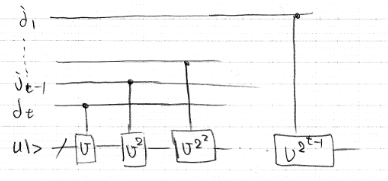
\includegraphics{Chapter 5/img5.7.png}
    
    \label{fig:my_label}
\end{figure}

Total number of $U$ operations is

$$ = 2^0 \times j_t + 2^1 j_{t-1} + 2^2 j_{t-2} +...+ 2^{t-1}j_1 = j$$



\paragraph{5.8} \textbf{Phase Estimation}
\\Solution attached as an image
\begin{figure}[h!]
    \centering
    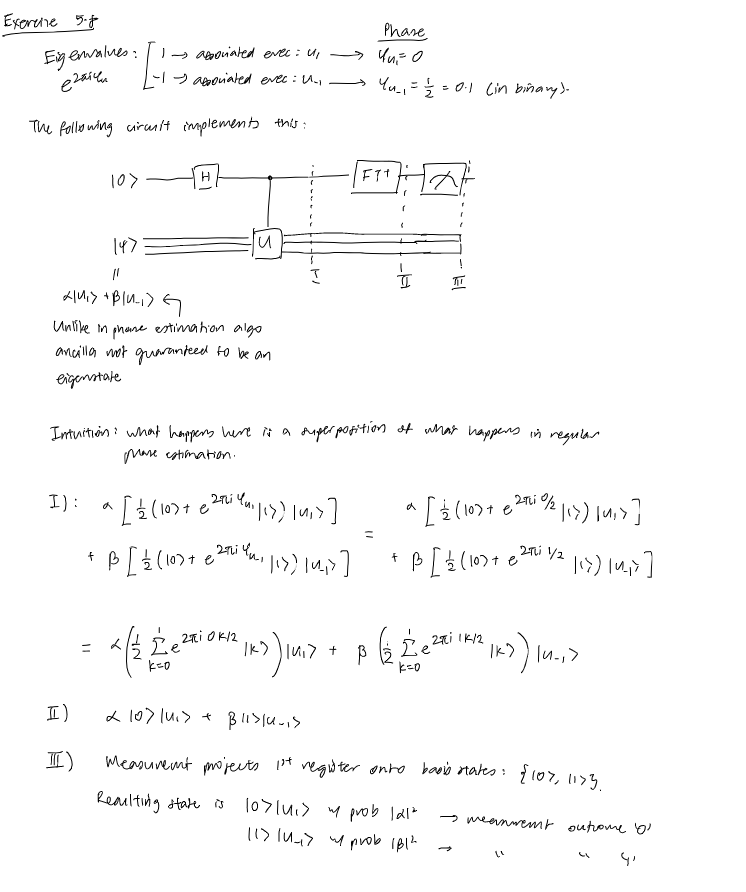
\includegraphics[width = \linewidth]{Chapter 5/Ex 5.8 soln.png}
    \caption{Solution to Exercise 5.8}
    \label{fig:my_label}
\end{figure}



\paragraph{5.9} \textbf{U be a unitary transform}
\\

Considering the case of $t=1$ in the phase estimation $\mu$

$$ \mu |0\rangle \otimes |u\rangle = \frac{1}{\sqrt{2}} \bigg( |0\rangle + e^{2 \pi \iota \phi} |1\rangle \bigg) \otimes |u\rangle$$

For,
$$|\phi\rangle = \alpha_{+} |\mu_{+}\rangle + \alpha_{-} |\mu_{-}\rangle $$

$$\mu|0\rangle \otimes |\phi\rangle = \frac{\alpha_+}{\sqrt{2}} \bigg( |0\rangle +|1\rangle \bigg) \otimes |\mu_+\rangle$$
$$ + \frac{\alpha_-}{\sqrt{2}} \bigg( |0\rangle -|1\rangle \bigg) \otimes |\mu_-\rangle $$

$$ (H \otimes 1) \cdot \mu (|0\rangle \otimes |\phi\rangle ) = \alpha_+ |0\rangle \otimes |\mu_+\rangle$$
$$+ \alpha_- |1\rangle \otimes |\mu_-\rangle$$

This is exactly the same circuit as in Ex 4.34


\paragraph{5.10} \textbf{Show that the order of } $x = 5 \text{ modulo } N = 21 \text{ is } 6$
\\

$$5^2 = 4 (\text{ mod } 21)$$
$$ 5^3 = 20( \text{ mod } 21)$$
$$ 5^4 = 100 = 16 (\text{ mod } 21)$$
$$ 5^5 = 80 = 19(\text{ mod } 21)$$
$$ 5^6 = 85 = 1(\text{ mod } 21)$$

\paragraph{5.11} \textbf{Show that the order of } $x$ satisfies $ r\le N$
\\

$\phi(n) :$  Euler function $ x^{\phi(n)} = 1 (\text{ mod } N)$

$$ r \le \phi(n) <  N$$

\paragraph{5.12} \textbf{Show that U is unitary}
\\
\begin{figure}[h!]
    \centering
    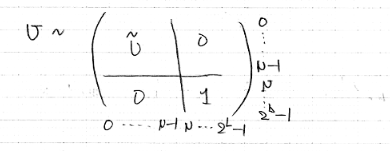
\includegraphics{Chapter 5/5.12.png}
    
    \label{fig:my_label}
\end{figure}
It is sufficient to show that $\tilde{U}^{\dagger} U = 1$

$$ 0 \le y,  y^{\prime} \le N-1$$
$$ \langle y^{\prime} | U^{\dagger} U|y\rangle = \langle x y^{\prime} | xy\rangle$$

if $xy^{\prime} = xy (\text{ mod } N)$
$$ \implies y^{\dagger} = y (\text{ mod } N)$$
$x$ is co-prime to $N$, so
$$ U^{\dagger} U = 1$$

\paragraph{5.13} \textbf{Prove 5.44}
\\

$$ \frac{1}{\sqrt{r}} \sum_{s=0}^{r-1} e^{2 \pi \iota s k/r} |u_s\rangle $$
$$ \frac{1}{r} \sum_{s \cdot k^{\prime} =0}^{r-1} e^{\frac{- 2 \pi \iota s(k^{\prime} -k)}{r}} |x^{k^{\prime}} \text{ mod } N\rangle$$

Now, 
$$\sum_{s=0}^{r-1} e^{\frac{-2 \pi \iota s (k^{\prime}-k)}{r}} = r (\text{ for } k^{\prime} = k)$$

$$ = \frac{1-e^{-2\pi \iota r (k^{\prime}-k)/r}}{1-e^{-2\pi \iota  (k^{\prime}-k)/r}} = 0$$
for $k^{\prime} = k$

$$ \Phi = \sum_{k^{\prime}=0}^{r-1} \delta_{k k^{\prime}} |x^{k^{\prime}} \text{ mod } N \rangle = |x^{k} \text{ mod } N\rangle$$

\paragraph{5.15} \textbf{}
\\

The least common multiple (LCM) of two positive integers x and y is the smallest positive integer that is a multiple of both x and y. The greatest common divisor (GCD) of x and y is the largest positive integer that divides both x and y without leaving a remainder.

We can use the property that the product of the LCM and GCD of two integers is equal to the product of the integers themselves:

$$ LCM(x,y) \times GCD(x,y) = x \times y $$

By dividing both sides of the equation by $GCD(x,y)$, we can find that:

$$LCM(x,y) = (x \times y) / GCD(x,y)$$

The GCD of two integers can be computed using the Euclidean algorithm in $O(L)$ operations, where L is the number of bits in the larger of the two integers. Therefore, computing the LCM of two L-bit integers using the formula above takes $O(L)$ operations for the GCD calculation and O(1) operations for the division, for a total of $O(L)$ operations.

It should be $O(L^2)$ instead of $O(L)$

\paragraph{5.20} \textbf{}
\\

Using the cyclicity:
$$ f(l) = \frac{1}{\sqrt{N}} \sum_{x=0}^{N-1} e^{-2 \pi \iota l x/N} f(x)$$
$$ \frac{1}{\sqrt{N}} \sum_{k=0}^{m-1} \sum_{x=0}^{r-1} e^{-2 \pi \iota  l (kr + x)/mr} f(x) $$

Now,
$$ \sum_{k=0}^{m-1} e^{-2 \pi \iota l k r /mr} = m \cdot \alpha e \cdot mn$$
$$ = \frac{\sqrt{N}}{r} \sum_{x=0}^{r-1} e^{- 2 \pi \iota l x /N} f(x) \alpha e \frac{N}{r}\times x$$

Especially for $N = r$

$$ f(l) = \frac{1}{\sqrt{r}} \sum_{x=0}^{r-1} e^{- 2 \pi \iota l x/ r} f(x)$$


\paragraph{5.21} \textbf{Period finding and phase estimation}
\\
\begin{figure}[h!]
    \centering
    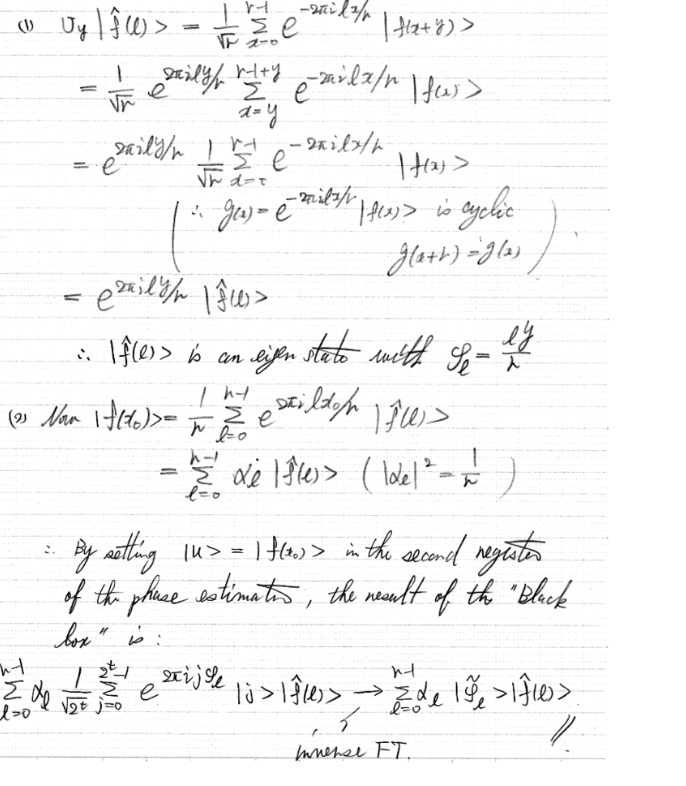
\includegraphics{Chapter 5/Ex 5.21 soln.png}
    \caption{5.21 solution}
    \label{fig:my_label}
\end{figure}

\paragraph{5.22} \textbf{}
\\
\begin{figure}[h!]
    \centering
    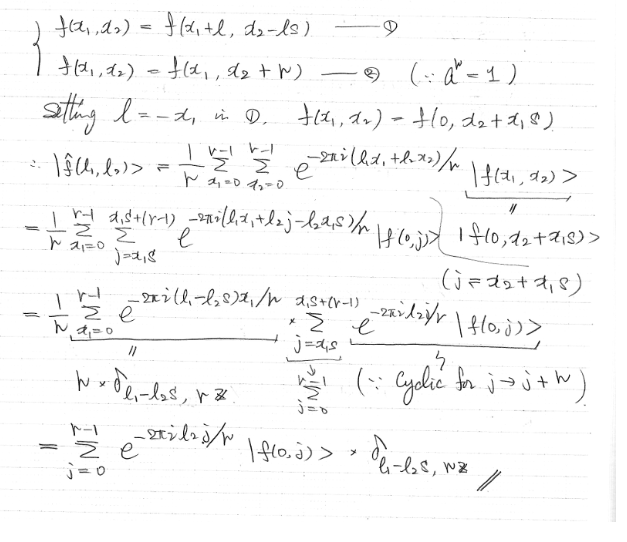
\includegraphics{Chapter 5/Ex 5.22 soln.png}
    \caption{5.22 solution}
    \label{fig:my_label}
\end{figure}

\paragraph{5.23} \textbf{}
\\
\begin{figure}[h!]
    \centering
    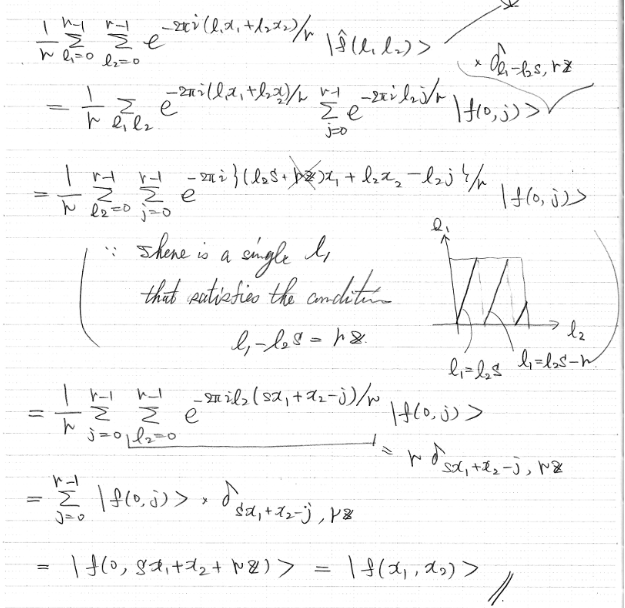
\includegraphics{Chapter 5/Ex 5.23 soln.png}
    \caption{5.23 solution}
    \label{fig:my_label}
\end{figure}
